\documentclass[final]{beamer}
% http://tex.stackexchange.com/questions/56205/wrapfigure-beamer-style
\usepackage{color}
\usepackage{transparent}
%\usepackage{cutwin}
%\usetheme{RJH}
\usetheme{Berkeley}
%\usetheme{Bergen}
\usepackage[orientation=portrait,size=a0,scale=1.4,debug]{beamerposter}
\usepackage[absolute,overlay]{textpos}
\setlength{\TPHorizModule}{1cm}
\setlength{\TPVertModule}{1cm}
\beamertemplatenavigationsymbolsempty
% RGB (145,201,219), #91C9DB
%\definecolor{mybluelabel}{RGB}{145,201,219}
% RGB (48,174,228), #30AEE4
\definecolor{mybluelabel}{RGB}{48,174,228}

\begin{document}
\begin{frame}{} 

%\begin{textblock}{20}(2,2)
%\begin{center}
%\begin{figure}[tbph]
%\centering
%%\includegraphics[width=0.45\textwidth]{dianahep-logo.png}
%
\includegraphics[width=0.70\textwidth]{images/diana-hep-06-logo-horizontal.png}
%\end{figure}
%\url{http://s2i2-hep.org}
%\end{center}
%\end{textblock}



\begin{textblock}{84.0}(1,2)
\begin{center}
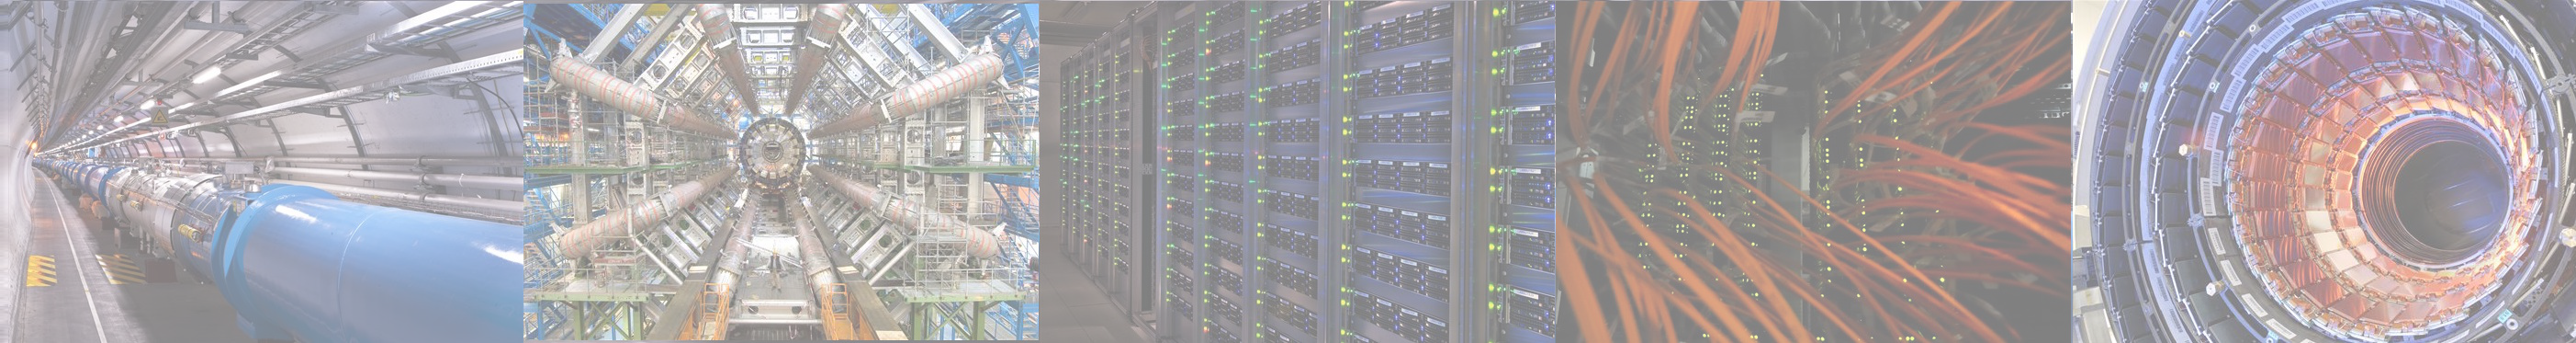
\includegraphics[width=0.95\textwidth]{images/s2i2-banner-50percent.png}
\end{center}
\end{textblock}

\begin{textblock}{84.0}(1,3)
\begin{center}
\begin{Huge}
%\color{white}{
\textbf{
Conceptualization of an S2I2 Institute \\
~~for High Energy Physics (S2I2-HEP)
}
%}
\end{Huge}
\end{center}
\end{textblock}

\begin{textblock}{84.0}(2,8.8)
\begin{center}
\begin{Large}
\textbf{
PIs: Peter Elmer (Princeton Univ.), Mark Neubauer (Univ. of Illinois \\ 
at Urbana-Champaign), Mike Sokoloff (Univ. of Cincinnati)
}
\end{Large}
\end{center}
\end{textblock}

\begin{textblock}{78.0}(4,14)
\begin{block}{The S2I2-HEP Project}
The primary goal of the S2I2-HEP conceptualization project is to
prepare a strategic plan for a potential NSF Scientific Software
Innovation Institute (S2I2) to develop software for experiments
taking data in the ``High-Luminosity Large Hadron Collider'' (HL-LHC)
era in the 2020s. In addition, we are working with the HEP Software
Foundation to prepare a larger HEP Community White Paper (CWP)
describing a global roadmap for HEP Software and Computing R\&D for
the 2020s. To this end we are organizing a number of workshops
between Fall 2016 and Summer 2017.
\end{block}
\end{textblock}

\begin{textblock}{38.0}(4,23.5)
\begin{block}{High Energy Physics (HEP)}
%\begin{center}
The quest to understand the fundamental building blocks of nature,
and their interactions, is one of the longest running and most
ambitious of human endeavors. Facilities such as the Large Hadron
Collider (LHC), where we do our research, represent a huge step
forward in our ability to answer these questions. The discovery of
the Higgs boson, the observation of exceedingly rare decays of B
mesons, and exclusion of countless theories beyond the Standard
Model (SM) of particle physics demonstrate that these experiments
deliver results. However, the most interesting fundamental physics
questions remain wide open, amongst them: What is the dark matter
which pervades the universe? Does space-time have additional
symmetries or extend beyond the 3 spatial dimensions we know? What
is the mechanism stabilizing the Higgs mass from enormous quantum
corrections? Are neutrinos, whose only SM interactions are weak,
their own anti-particles? Can the theories of gravity and quantum
mechanics be reconciled? Planned and running HEP experiments 
aim to answer these questions over the next 20 years. 
XXXXX In addition to the large facilities (accelerators and large particle
detectors), the computing and software challenges 
are formidable. XXXX
The LHC experiments, for example, use nearly 0.5 Exabyte of
storage today in 170 computer centers in 42 countries. 
The upgrade to the High-Luminosity Large Hadron Collider (HL-LHC) will
increase the data volume
by more than a factor of 100, with significantly increased data and detector complexity. The resulting computing needs will outpace the expected improvements in computer performance (Moore's Law) by factors of between 3 and 30. 

\begin{figure}[tbph]
\centering
%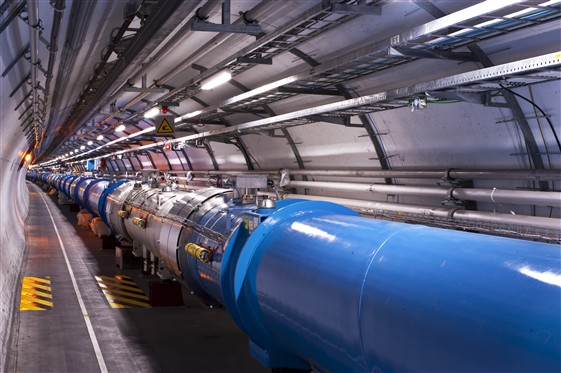
\includegraphics[width=0.48\textwidth]{images/0910152_02-A5-at-72-dpi.jpg}
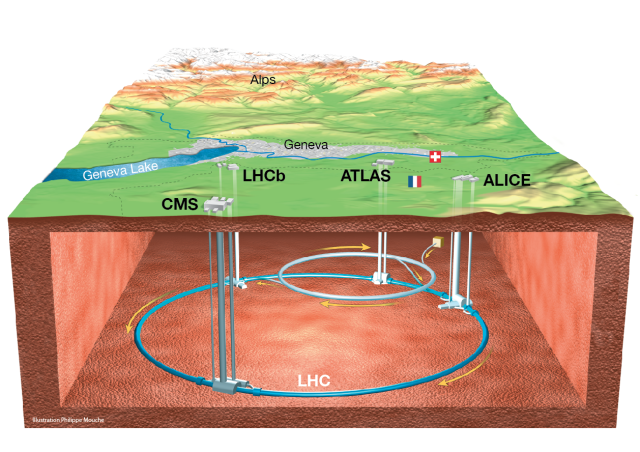
\includegraphics[width=0.41\textwidth]{images/CERN-LHC-cutaway-view-medium.png}
%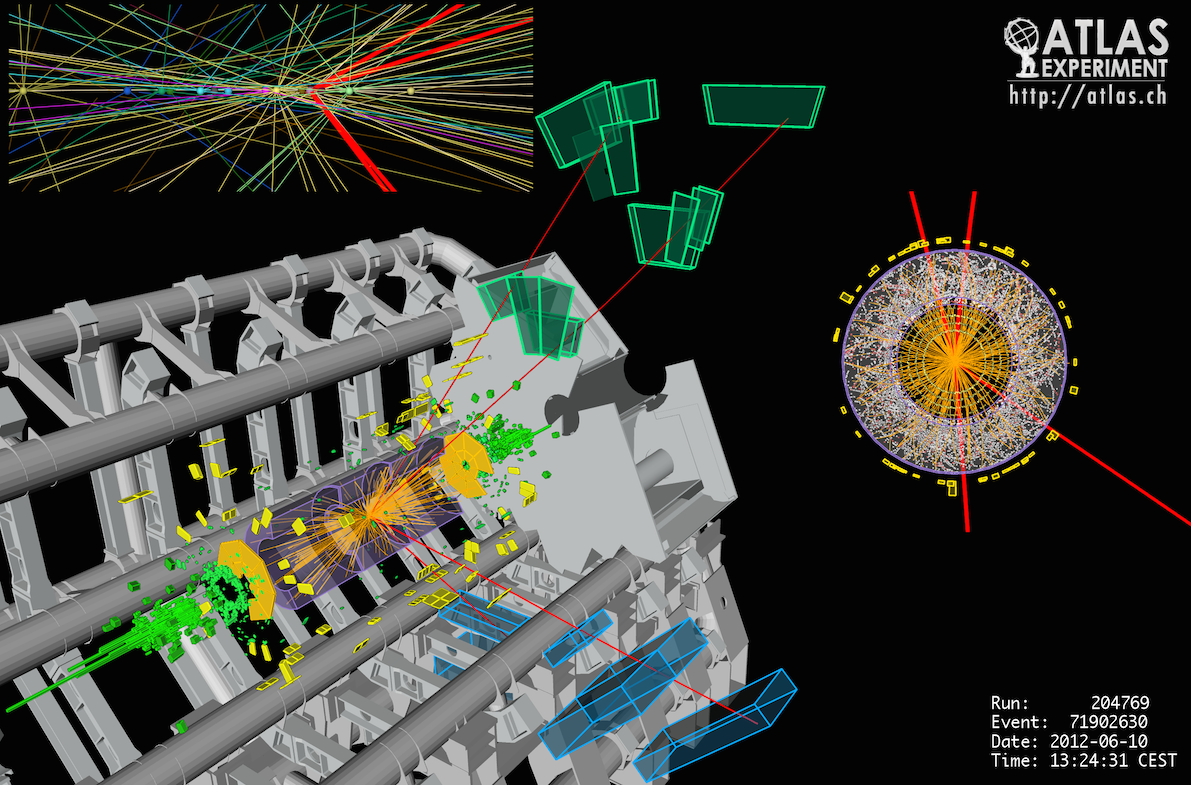
\includegraphics[width=0.41\textwidth]{images/run204769_evt71902630_VP1Base-half.png}
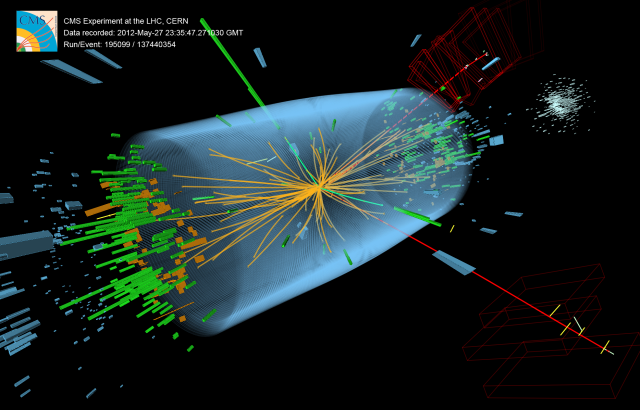
\includegraphics[width=0.42\textwidth]{images/eemm_run195099_evt137440354_ispy_3d-annotated-2.png}
%\begin{center}
%\end{center}
\end{figure}
{\small \copyright~2009-2016 CERN (License: CC-BY-SA-4.0)}
\end{block}
\end{textblock}

%\begin{textblock}{38.0}(4,65)
%\begin{block}{High-Luminosity Large Hadron Collider (HL-LHC)}
%\end{block}
%\end{textblock}


\begin{textblock}{38.0}(4,75)
\begin{block}{The HEP Community and Software Ecosystem}
HEP collaborations, US scientists/students involved in LHC, etc. (Additional text to fill in.)

The aim of the CWP is  to identify and prioritise the software research and development investments required:

\begin{itemize}
\item to achieve improvements in software efficiency, scalability and performance and to make use of the advances in CPU, storage and network technologies
\item to enable new approaches to computing and software that could radically extend the physics reach of the detectors
\item to ensure the long term sustainability of the software through the lifetime of the HL-LHC
\end{itemize}


\end{block}
\end{textblock}




\begin{textblock}{38.0}(44,23.5)
\begin{block}{S2I2 HEP/CS workshop at NCSA, 7-9 Dec 2016}
The first S2I2-HEP workshop focused on fostering collaboration between the HEP and Computer Science communities. There were 50 attendees, with about half from HEP and half from Computer Science.
\begin{figure}[tbph]
\centering
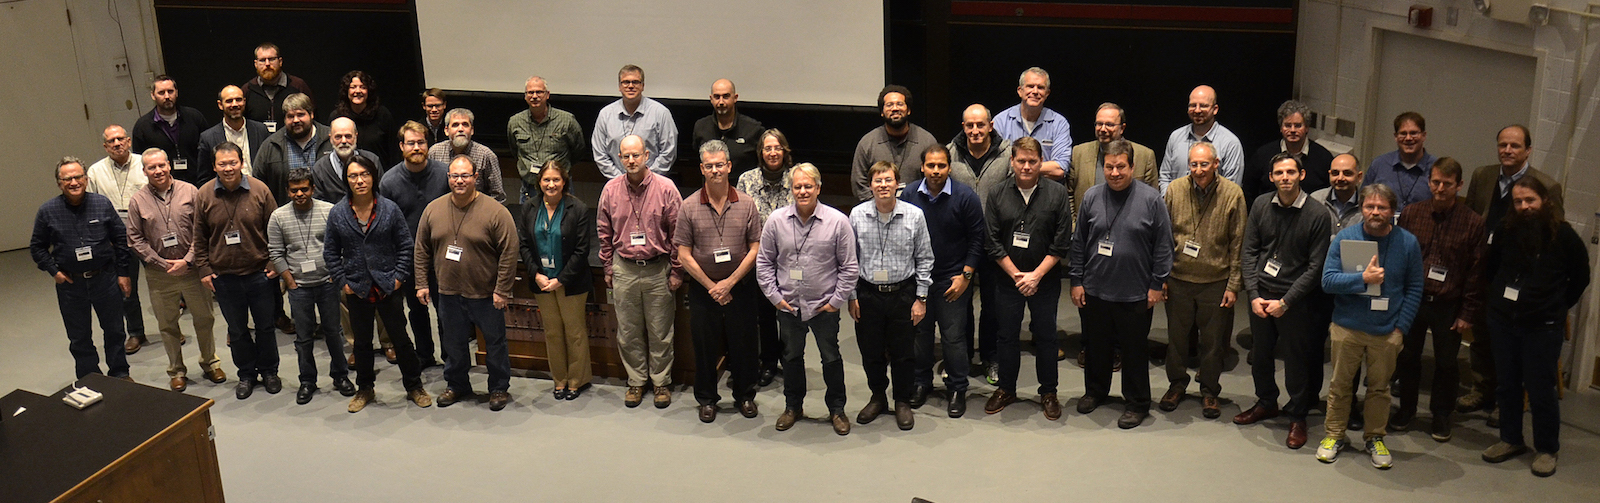
\includegraphics[width=0.60\textwidth]{images/20161208-s2i2-hep-cs-group-photo.jpg}
\end{figure}
\small{Meeting agenda: \url{https://indico.cern.ch/event/575443/}} \\
\small{Summary: \url{http://s2i2-hep.org/downloads/s2i2-hep-cs-workshop-summary.pdf}}
\end{block}
\end{textblock}

\begin{textblock}{38.0}(44,42)
\begin{block}{HSF Community White Paper Workshop at SDSC, 23-26 Jan 2017}
This was the first CWP workshop, organized jointly by S2I2-HEP and the HEP Software Foundation (\url{http://hepsoftwarefoundation.org}). The aim of this workshop was to begin the CWP process, formulate charges and plans for the CWP working groups. It consisted of plenary sessions, parallels and topical panels with 120 attendees from HEP, Computer Science and Industry.
\begin{figure}[tbph]
\centering
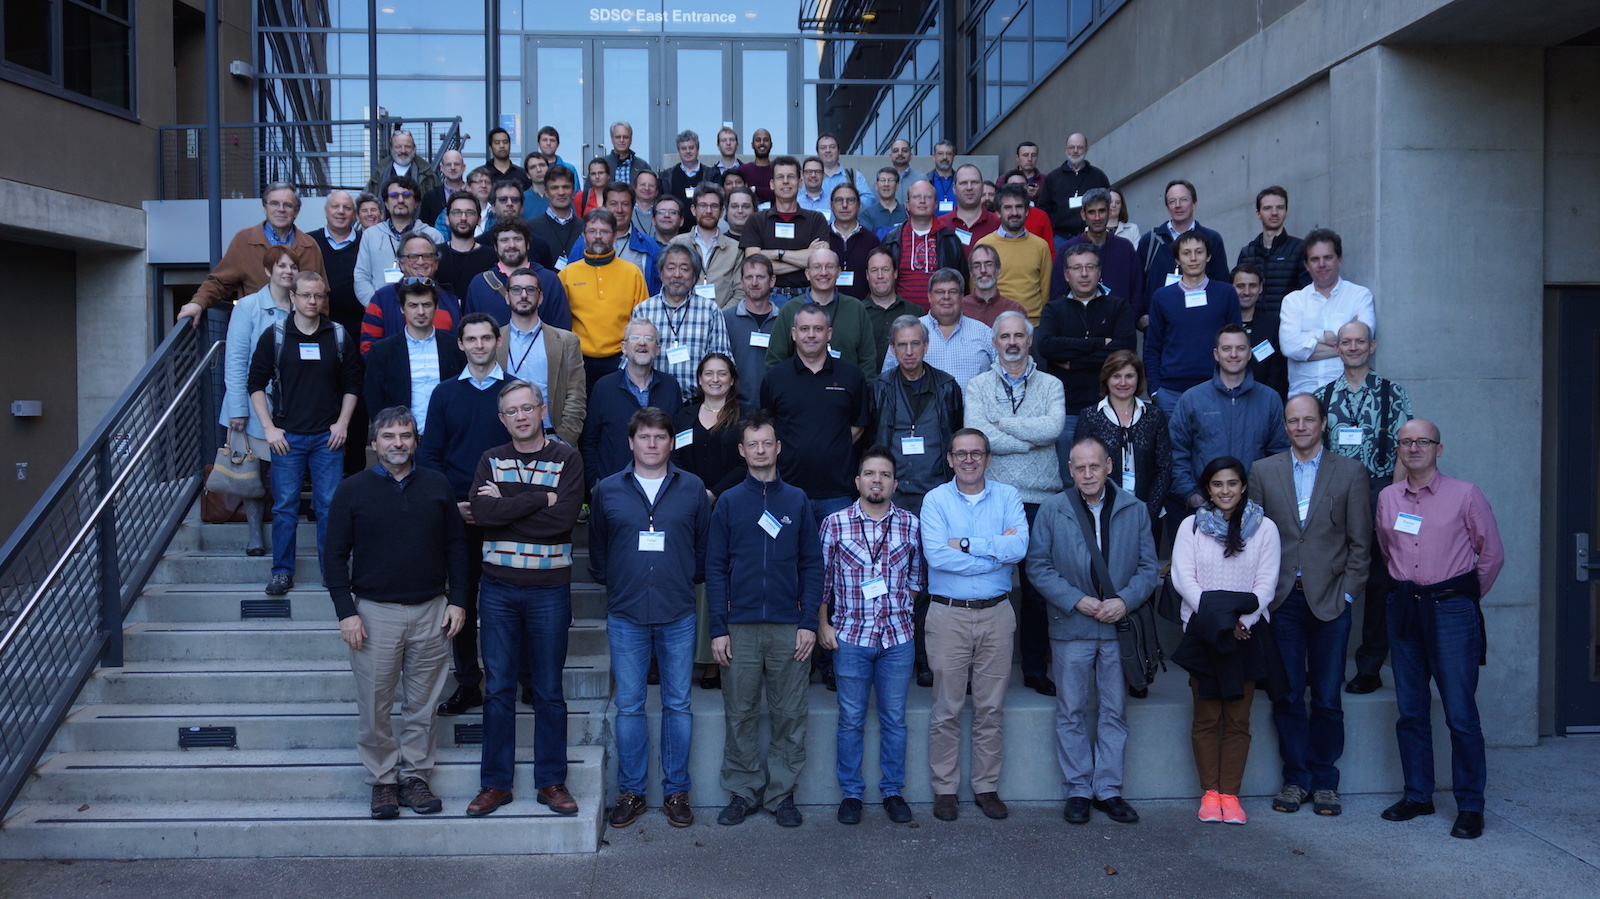
\includegraphics[width=0.50\textwidth]{images/20170125-HSF-SDSC-Workshop-group-photo.jpg}
\end{figure}
Topics covered included simulation, data analysis and interpretation, event processing frameworks, workflow and resource management, triggering and reconstruction, data analytics and machine learning, data access and management, visualization, data and software preservation and software development, deployment and validation. \\
\small{Meeting agenda: \url{http://indico.cern.ch/event/570249/}} \\

\end{block}
\end{textblock}

\begin{textblock}{38.0}(44,73)
\begin{block}{Future S2I2-HEP and HSF/CWP activities}
We are planning additional CWP workshops are planned this year: \\
\begin{itemize}
\item 9 Mar, 2017 - Software Triggers and Event Reconstruction WG meeting
    \begin{itemize}
    \item LAL (Orsay)
    \item Session at the Connecting The Dots workshop (\url{https://ctdwit2017.lal.in2p3.fr})
    \item Indico page: \url{https://indico.cern.ch/event/614111/}
    \end{itemize}
\item 20-22 Mar, 2017 - IML Topical Machine Learning Workshop
    \begin{itemize}
    \item CERN
    \item The workshop includes a CWP session on Machine Learning
    \item Indico page: \url{https://indico.cern.ch/event/595059}
    \end{itemize}
\item 22-24 May, 2017 - HEP Analysis Ecosystem Retreat
    \begin{itemize}
    \item Location TBD
    \item Indico page: \url{http://indico.cern.ch/event/613842/}
    \item Workshop proposal: \url{http://goo.gl/mbvAUT}
    \end{itemize}
\item 5-6 Jun, 2017 - CWP Event Processing Frameworks Workshop (TBC)
    \begin{itemize}
    \item FNAL
    \item The workshop is just prior to the FNAL 50th Anniversary and User Meeting
    \end{itemize}
\item 26-30 Jun, 2017 - HEP Software Foundation Workshop
    \begin{itemize}
    \item LAPP (Annecy)
    \item Final CWP workshop
    \item Indico page: \url{https://indico.cern.ch/event/613093/}
    \end{itemize}
\end{itemize}
In addition we are investigating the possibility of a 2nd S2I2 HEP/CS workshop in May at Princeton (TBC) and a possible S2I2-HEP meeting at the ACAT 2017 conference in Seattle the week of 21-25 Aug, 2017.
\end{block}
\end{textblock}










\begin{textblock}{14.0}(4,109)
\begin{block}{This poster online with links}
\begin{figure}[tbph]
\centering

\includegraphics[width=0.30\textwidth]{images/qr-s2i2-hep-si2-pi-workshop-2017.png}
\end{figure}
\begin{center}
\url{http://goo.gl/k22mD9}
\end{center}
\end{block}
\end{textblock}


\begin{textblock}{14.0}(20,109)
\begin{block}{S2I2-HEP Project website}
\begin{figure}[tbph]
\centering

\includegraphics[width=0.30\textwidth]{images/qr-s2i2-hep.png}
\end{figure}
\begin{center}
\url{http://s2i2-hep.org}
\end{center}
\end{block}
\end{textblock}



\begin{textblock}{38.0}(44,109)
\begin{block}{Acknowledgement}
This project is supported by National Science Foundation grants ACI-1558216, ACI-1558219, and ACI-1558233. Any opinions, findings, conclusions or recommendations expressed in this material are those of the developers and do not necessarily reflect the views of the National Science Foundation. \\
%~~\\
%\begin{center}
%Images \copyright~2009-2016 CERN (License: CC-BY-SA-4.0)
%\end{center}

\end{block}
\end{textblock}




\end{frame}
\end{document}
